\documentclass[a4paper]{jsarticle}%pLatexでコンパイルしてください
\usepackage{ml2.2}

\begin{document}
\maketitle
%%%概要を出力したい人はこのように記述
\vspace{-0.4cm}
\begin{figure}[H] 
  \centering
  \begin{tikzpicture}[remember picture, overlay]
      \node[anchor=north east] at (current page.north east) {
          
\includegraphics[width=2cm]{pics/qr.png} 
      };
      \node[anchor=north east, yshift=-2cm] at (current page.north east) {デジタル版はここ};
  \end{tikzpicture}
  \label{fig:my_label}
\end{figure}
\section{\textbf{Sigmoidal Function}}
\thispagestyle{plain}
\begin{dfn}[シグモイド関数]
\addcontentsline{toc}{subsubsection}{定義}
Logistic関数 $\sigma(x):\mathbb{R}\to [0,1] $ は、次のように定義される。
\begin{equation}
  \sigma(x) = \frac{1}{1 + e^{-x}} \quad (x \in \mathbb{R})\label{eq1}
\end{equation}
式\eqref{eq1}によって、$\displaystyle\lim_{x\to -\infty}\sigma(x)=0$,$\quad\displaystyle\lim_{x\to +\infty}\sigma(x)=1$となる。\\
上の条件を満たすような関数をシグモイド関数と言う。\\
\begin{figure}[h]
  \centering
  \begin{minipage}{0.43\columnwidth}
    \centering
    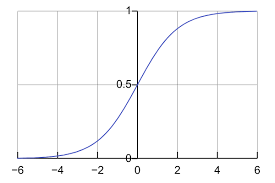
\includegraphics[width=\columnwidth]{pics/p1.2.png}
    \caption{Logistic関数}
    \label{fig:p1}
  \end{minipage}
  \hspace{5mm}
  \begin{minipage}{0.43\columnwidth}
    \centering
    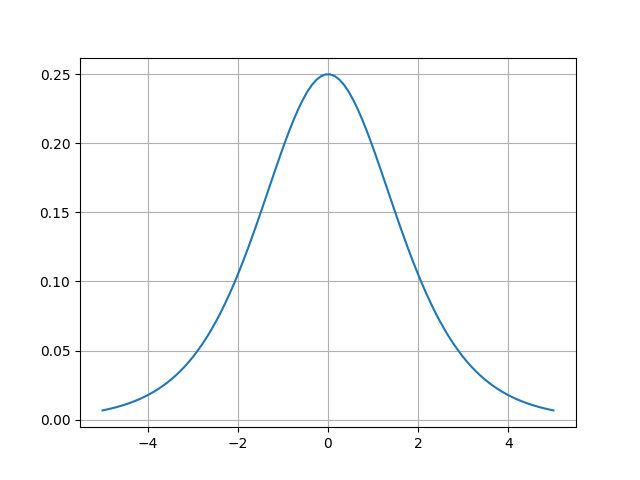
\includegraphics[width=\columnwidth]{pics/p1.1.png}
    \caption{Logistic関数の1階微分}
    \label{fig:p2}
  \end{minipage}
\end{figure}
\begin{exercise}
  以上のLogistic関数が微分可能であることを示せ。
\end{exercise}

\begin{proof}
まず、関数の微分は次の定義によって与えられます:
\[
f'(x) = \lim_{h \to 0} \frac{f(x + h) - f(x)}{h}
\]
この定義を用いて、Logistic関数の微分を計算すると、次のようになります:\\
まず、\(f(x + h)\)と\(f(x)\)を計算します:
\[
f(x + h) = \frac{1}{1 + e^{-(x + h)}} = \frac{1}{1 + e^{-x} e^{-h}} = \frac{1}{1 + \frac{e^{-x}}{e^{h}}}
\]
次に、差 \(f(x + h) - f(x)\)を計算します:
\[
f(x + h) - f(x) = \frac{1}{1 + e^{-x} e^{-h}} - \frac{1}{1 + e^{-x}}
\]
この差を通分します:
\[
= \frac{(1 + e^{-x}) - (1 + e^{-x} e^{-h})}{(1 + e^{-x} e^{-h})(1 + e^{-x})}
= \frac{e^{-x} - e^{-x} e^{-h}}{(1 + e^{-x} e^{-h})(1 + e^{-x})}
\]

次に、これを微分の定義に代入します:
\[
f'(x) = \lim_{h \to 0} \frac{e^{-x}(1 - e^{-h})}{h(1 + e^{-x} e^{-h})(1 + e^{-x})}
\]
ここで、\(\lim_{h \to 0} \frac{1 - e^{-h}}{h} = 1\)\footnote{関数 \(e^{-h}\)のテイラー展開は以下のようになります:
\[
e^{-h} = 1 - h + \frac{h^2}{2!} - \frac{h^3}{3!} + \cdots
\]

したがって、\(1 - e^{-h}\)を考えると:
\[
1 - e^{-h} = h - \frac{h^2}{2!} + \frac{h^3}{3!} - \cdots
\]

\[
\frac{1 - e^{-h}}{h} = \frac{h - \frac{h^2}{2!} + \frac{h^3}{3!} - \cdots}{h}
\]
これを整理すると:
\[
  \frac{1 - e^{-h}}{h}= 1 - \frac{h}{2!} + \frac{h^2}{3!} - \cdots
\]
\(h\)が0に近づくと、右辺の高次の項(\(-\frac{h}{2!} + \frac{h^2}{3!} - \cdots\))は全て0に近づきます。したがって、
\[
\lim_{h \to 0} \frac{1 - e^{-h}}{h} =\lim_{h \to 0} \left(1 - \frac{h}{2!} + \frac{h^2}{3!} - \cdots\right) = 1
\]
}であることを用います。このため、別の形に表しましょう:
\[
f'(x) = e^{-x} \lim_{h \to 0} \frac{1 - e^{-h}}{h} \cdot \frac{1}{(1 + e^{-x} e^{-h})(1 + e^{-x})}
\]
$\lim_{h \to 0} \frac{1 - e^{-h}}{h} = 1 \quad \text{なので、これは次のようになります:}$
\[
f'(x) = e^{-x} \cdot \frac{1}{(1 + e^{-x})(1 + e^{-x})} = e^{-x} \cdot \frac{1}{(1 + e^{-x})^2}
\]
さらに、\(f(x)\)を使って展開します:
\[
f(x) = \frac{1}{1 + e^{-x}} \Rightarrow 1 - f(x) = \frac{e^{-x}}{1 + e^{-x}}
\]
したがって、次のように書けます:
\[
e^{-x} = (1 + e^{-x}) \cdot (1 - f(x))
\]
これらを微分の結果に代入すると:
\[
f'(x) = \frac{(1 + e^{-x})(1 - f(x))}{(1 + e^{-x})^2} = f(x)(1 - f(x))
\]

したがって、Logistic関数の微分は次のように表されます:
\[
f'(x) = f(x)(1 - f(x))
\]


\end{proof}
\end{dfn}

\begin{rem}
  測度 $\mu$ は情報を評価するために使われる判定のシステムとして扱うことができることを思い出してください。
  したがって、$d\mu(x) = \mu(dx)$ は、$x$ にインプットされた情報の評価を表します。
  結果として、積分 $\int f(x) d\mu(x)$ は、判定のシステム $\mu$ の下での関数 $f(x)$ の評価を表します。
  
\end{rem}
\section{\textbf{Discriminatory Function}}

\begin{dfn}[Discriminatory Function]
  この定義は、区別関数(Discriminatory Function)の概念を導入します。
  これは以下の特性によって特徴づけられます。
  すなわち、ニューロンの出力の評価 $\sigma(\mathbf{w}^T x + \theta)$ が、任意の入力 $x$ に対して、測度 $\mu$ の下で、任意の閾値 $\theta$ と任意の重み $\mathbf{w}$ に対してなくなると、$\mu$ も絶対なくなる。
  つまり、$\mu$ は無効な測度です。\\
  次に、測度$\mu \in M(I_n)$ とします。関数 $\sigma$ が測度 $\mu$ に対して区別的であるとは、次の条件を満たす場合に呼ばれます:

  \[
  \int_{I_n} \sigma(\mathbf{w}^T x + \theta)d\mu(x) = 0, \, \forall \mathbf{w} \in \mathbb{R}^n, \, \forall \theta \in \mathbb{R} \Rightarrow \mu = 0.
  \]
  ここで、関数 $\sigma$ は必ずしもLogistic関数である必要はなく、必要な特性を満たす任意の関数で構いません。
  $\mathcal{P}_{\mathbf{w},\theta} = \{x; \mathbf{w}^T x + \theta = 0\}$ を法線ベクトル $\mathbf{w}$ と $(n+1)$ 次の切片 $\theta$ を持つ超平面(hyperplane)とします。また、開半空間(open half-space)を次のように定義します。
  \[
  \mathcal{H}_{\mathbf{w},\theta}^+ = \mathcal{H}_{\mathbf{w},\theta} = \{x; \mathbf{w}^T x + \theta > 0\}, \quad \mathcal{H}_{\mathbf{w},\theta}^- = \{x; \mathbf{w}^T x + \theta < 0\}
  \]
従って、$\mathbb{R}^n = \mathcal{H}_{\mathbf{w},\theta}^+ \cup \mathcal{H}_{\mathbf{w},\theta}^- \cup \mathcal{P}_{\mathbf{w},\theta}$ となる。
\end{dfn}

\begin{dfn}[Baire測度]
Baire測度はBaire集合族\footnote{$ K\subset \mathbb{R}^{n}とし,\mathbf{Baire}集合族 \mathcal{B}とは, f\in C^{0}(K)=\{f\in C^{0}(K)|Supp\ f\ is\ compact\}に対し,\{x;f(x)\geq a\}の形で生成される \mathcal{\sigma-代数}として定義される。
そのSuppを関数の台と言い、位相空間でK\subset \mathbb{R}^{n}とし、f:\ K\rightarrow \mathbb{R}(or\ \mathbb{C})について、関数の台とは、Supp\ f\coloneqq \overline{\{x\in K|f(x)\not = 0\}}=\overline{(K-f^{-1}(0))}\ (ただし上付きバーは閉包(Closure)を表す) $} $ \mathcal{B} $,\ 
$K\subset \mathbb{R}^{n}$とし,Baire測度 $ \mu : \mathcal{B}\rightarrow [0,\infty]\ (or\ [0,\infty)\cup\{\infty\})\quad s.t.\ \forall C\subset K\ is\ compact,\ \mu (C)<\infty 。$
なお、$K\subset \mathbb{R}^{n}$ のとき、Baire集合族はBorel集合族と一致する。特に、任意の有限Borel測度はBaire測度である。
\end{dfn}
次に、$I_n = [0, 1]^n = [0, 1] \times \cdots \times [0, 1]$ としたとき、$I_n$ 上の有限の符号付き正則Baire測度の空間を $M(I_n)$ とする.
\begin{lem}
 $\mu \in M(I_n)$ とします。もし $\mu$ がすべての超平面と $\mathbb{R}^n$ の開半空間で0になるなら、$\mu$ は0です。すなわち、以下が成り立つとき、

\[
\mu(P_{\mathbf{w},\theta}) = 0, \quad \mu(\mathcal{H}_{\mathbf{w},\theta}) = 0, \quad \forall \mathbf{w} \in \mathbb{R}^n, \, \theta \in \mathbb{R},
\]
そのとき $\mu = 0$ です。
\pagebreak

\begin{exercise}
  \[
\mu(P_{\mathbf{w},\theta}) = 0, \quad \mu(\mathcal{H}_{\mathbf{w},\theta}) = 0, \quad (\forall \mathbf{w} \in \mathbb{R}^n, \, \theta \in \mathbb{R})\implies \mu = 0.\]
上記の補題を証明せよ。
\end{exercise}

\begin{proof} 
$\mathbf{w} \in \mathbb{R}^n$ を固定します。次のように定義された線形関数 $F : L^\infty(\mathbb{R})\footnotemark \to \mathbb{R}$ を考えます。
\footnotetext{実数集合 $\mathbb{R}$上で、$L^{\infty}(\mathbb{R})$ は「本質的に有界な」可測関数によって構成される空間である。$f \in L^{\infty}(\mathbb{R})$ に対して、そのノルムを
\[
\|f\|_{\infty} = \operatorname{ess\,sup}_{x \in \mathbb{R}} |f(x)| = \inf\{M : |f(x)| \leq M \text{ a.e.}\}
\]
と定義する。このノルムはバナッハ空間の三角不等式を満たし、また $L^{\infty}(\mathbb{R})$ を完備ノルム空間(すなわちバナッハ空間)にする。}
\[
F(h) = \int_{I_n} h(\mathbf{w}^T x) d\mu(x),
\]
ここで $L^\infty(\mathbb{R})$ はほぼ至る所($\mathrm{almost\ everywhere}\iff$ a.e.)で有界な関数の空間を表します。\\
$L^{\infty}(\mathbb{R})$ の元 $h$ は、$\mathbb{R}$ 上の有界な関数であり、$||h||_\infty = \text{ess}\displaystyle\sup_{x \in \mathbb{R}} |h(x)|\footnote{ess supを本質的上限と呼ばれ、定義は以下のようになります。
\[
(X,\mathcal{A},\mu) \text{ を測度空間, } f:X \to \mathbb{R} \text{ を可測関数とする. このとき,}
\quad\text{ess } \sup f = \inf \{ a \in \mathbb{R} \mid \mu(f > a) = 0 \}\]}
<\infty$ で定義されます。\\
$h\leq ||h||_\infty$ により、
\[
|F(h)| = \left| \int_{I_n} h(\mathbf{w}^T x) d\mu(x) \right| \leq ||h||_\infty \left|\int_{I_n} d\mu(x)\right| =  |\mu(I_n)| \cdot ||h||_\infty 
\]
ここで $\mu$ が有限測度である。
次に $h = 1_{[\theta,\infty)}$ とします。すなわち、$h$ は区間 $[\theta,\infty)$ の指示関数\footnote{指示函数(indicator function)または特性関数(characteristic function)\ $1_{[\theta,\infty)}(x)$の定義は
\[
1_{[\theta,\infty)}(x) = 
\begin{cases}
1, & x \geq \theta \\

0, & x < \theta
\end{cases}
\]}であり、$\mathbf{w}^T x\geq\theta$。すると、


\begin{align}
  F(h) = \int_{I_n} h(\mathbf{w}^T x) d\mu(x) &= \int_{\{\mathbf{w}^T x \geq \theta\}} \mathbf{1} d\mu(x)  +\int_{\{\mathbf{w}^T x < \theta\}} 0d\mu(x) \notag\\
  &= \int_{\{\mathbf{w}^T x \geq \theta\}} \mathbf{1}d\mu(x) + 0 \notag\\
  &=\mu(\mathcal{P}_{\mathbf{w},\theta}\cup\mathcal{H}_{\mathbf{w},\theta}^+) \notag\\
  &= \mu(\mathcal{P}_{\mathbf{w},\theta}) + \mu(\mathcal{H}_{\mathbf{w},\theta}^+)\footnotemark\notag\\
  &= 0\notag
\end{align}
\footnotetext{測度$\mu$の測度の性質の有限加法性によるためである.}
同様に$h = 1_{(\theta,\infty)}$を考えると、

\begin{align}
  F(h) = \int_{I_n} h(\mathbf{w}^T x) d\mu(x) &= \int_{\{\mathbf{w}^T x > \theta\}} d\mu(x)+\int_{\{\mathbf{w}^T x \leq \theta\}} d\mu(x)\notag \\
  &= \mu(\mathcal{H}_{\mathbf{w},-\theta}) \notag\\
  &= 0\notag
\end{align}
指示函数$1_{[a,b]}(x)$の定義は
$$
1_{[a,b]}(x) = 
\begin{cases}
1, & x \in [a,b] \\

0, & x \notin [a,b]
\end{cases}
$$
\boxed{\textbf{閉区間の場合:}}

\[
1_{[a,b]}(x) = 1_{[a,\infty)}(x) - 1_{(b,\infty)}(x).
\]
確認すると、

\begin{itemize}
    \item \textbf{ $x < a$ の時:}
    \begin{align*}
    1_{[a,\infty)}(x) &= 0, \\
    1_{(b,\infty)}(x) &= 0,\\
    1_{[a,\infty)}(x) - 1_{(b,\infty)}(x) &= 0, \quad \text{指示関数として定義。}
    \end{align*}

    \item \textbf{ $a \leq x \leq b$ の時:}
    \begin{align*}
    1_{[a,\infty)}(x) &= 1, \\
    1_{(b,\infty)}(x) &= 0,\\
    1_{[a,\infty)}(x) - 1_{(b,\infty)}(x) &= 1, \quad \text{指示関数として定義。}
    \end{align*}

    \item \textbf{ $x > b$ の時:}
    \begin{align*}
    1_{[a,\infty)}(x) &= 1, \\
    1_{(b,\infty)}(x) &= 1,\\
    1_{[a,\infty)}(x) - 1_{(b,\infty)}(x) &= 0, \quad \text{指示関数として定義。}
    \end{align*}
\end{itemize}

同様に、\boxed{\textbf{開区間の場合:}}

\[
1_{(a,b)}(x) = 1_{[a,\infty)}(x) - 1_{(b,\infty)}(x).
\]

したがって、$F$の線形性\footnote{関数Fの線形性とは、$F(\alpha f+\beta g)=\alpha F(f)+\beta F(g) \quad (\alpha ,\beta\in \mathbb{R})$}より、次のように書けます。
\[
F\left(\sum_{i=1}^N \alpha_i 1_{J_i}\right) = \sum_{i=1}^N \alpha_i F(1_{J_i}) = 0,
\]
ここで $\alpha_i \in \mathbb{R}$、$J_i$ は区間です。単関数\footnote{\textbf{Appendix A}を参照してください}が $L^\infty(\mathbb{R})$ において稠密\footnote{位相空間 $X$ の部分集合 $A$ が $X$ において \textbf{稠密(Dense)} であるとは,
$X$ の各元 $x$ に対し,$x$ の任意の近傍が $A$ の元を少なくとも一つ含むことをいう。
同じことだが,$A$ が $X$ において稠密であるのは,
$A$ を含む $X$ の閉集合が $X$ 自身しかないときであり,かつそのときに限る。
これは $A$ の閉包 $\overline{A}$ が $X$ に一致すると言ってもよい。
あるいは,$A$ の補集合の内部が空であるともいえる。位相空間 $X$ の \textbf{稠密度(Density)} とは,
$X$ の稠密部分集合の最小濃度をいう。}であるため、$F' = 0$ が成り立ちます。よって、任意の固定された $f \in L^\infty(\mathbb{R})$ に対して、$(s_n)_n$ が存在して $s_n \to f\quad (n\to\infty)$ となります。
$F$ が有界かつ連続\footnote{連続関数ならば、関数記号と極限が交換可能である.その証明は$\displaystyle\epsilon - \delta$論法を使えば、簡単に証明できる}であるので、以下が成り立ちます。
\[
F(f) = F\left(\lim_{n \to \infty} s_n\right) = \lim_{n \to \infty} F(s_n) = 0.
\]

次に、測度 $\mu$ のフーリエ変換を計算すると。

\[
\hat{\mu}(\mathbf{w}) = \int_{I_n} e^{i \mathbf{w}^T x} d\mu(x) = \int_{I_n} \cos(\mathbf{w}^T x) d\mu(x) + i \int_{I_n} \sin(\mathbf{w}^T x) d\mu(x).\footnote{オイラーの公式:$e^{i\theta}=\cos(\theta)+i\sin(\theta)$}
\]

$F(\cos(\cdot))=\int_{I_n} \cos(\mathbf{w}^T x) d\mu(x),F(\sin(\cdot))=\int_{I_n} \sin(\mathbf{w}^T x) d\mu(x)$を用いて、$cos$と$sin$関数は全部有界関数なので、以下が成り立ちます。

\[
F(\cos(\cdot)) + i F(\sin(\cdot)) = 0, \quad \forall \mathbf{w} \in \mathbb{R}^n,
\]

フーリエ変換の単射\footnote{$f: X \to Y が$\text{が単射 (injective) であるとは,}
$\forall x_1, x_2 \in X, \quad x_1 \neq x_2 \implies f(x_1) \neq f(x_2)$

\text{となること。対偶をとっていいかえると,}
$f(x_1) = f(x_2) \implies x_1 = x_2$}性質から、$\mu = 0$ が成り立つ。
\end{proof}

  
\end{lem}




\begin{prop}
任意の連続シグモイド関数は、$M(I_n)$ のすべての測度 $\mu$ に対して区別可能である。


\begin{proof}
$\mu \in M(I_n)$ を固定された測度とする。以下の条件を満たす連続シグモイド $\sigma$ を選ぶ:
\begin{equation}
  \int_{I_n} \sigma(\mathbf{w}^T x + \theta)d\mu(x) = 0, \quad \forall \mathbf{w} \in \mathbb{R}^n, \theta \in \mathbb{R}.\label{eq2}
\end{equation}
$\mu=0$を証明すればいい。まず、以下の関数を構成すると、
\[
\sigma_\lambda(x) = \sigma(\lambda(\mathbf{w}^T x + \theta) + \phi)
\]

シグモイド関数の定義により:

\[
\lim_{\lambda \to \infty} \sigma_\lambda(x) = \begin{cases} 
1, & \text{if } \mathbf{w}^T x + \theta > 0 \\
0, & \text{if } \mathbf{w}^T x + \theta < 0 \\
\sigma(\phi), & \text{if } \mathbf{w}^T x + \theta = 0
\end{cases}
\]

境界関数 $\gamma(x)$ を定義すると

\[
\gamma(x) = \begin{cases} 
1, & \text{if } x \in \mathcal{H}^+_{\mathbf{w},\theta} \\
0, & \text{if } x \in \mathcal{H}^-_{\mathbf{w},\theta} \\
\sigma(\phi), & \text{if } x \in \mathcal{P}_{\mathbf{w},\theta}
\end{cases}
\]

$\sigma_\lambda(x) \to \gamma(x)\quad (\lambda\to\infty)$ は $\mathbb{R}^n$ 上で各点収束し、また $\sigma$ はシグモイド関数であるため、値は有限区間にある。
有界収束定理\cite{lang1993real}より、極限と積分の交換ができる。よって、
\begin{align}
  \lim_{\lambda \to \infty} \int_{I_n} \sigma_\lambda(x) d\mu(x) &= \int_{I_n} \gamma(x) d\mu(x)\notag\\
  &= \int_{\mathcal{H}^+_{\mathbf{w},\theta}} \gamma(x) d\mu(x) + \int_{\mathcal{H}^-_{\mathbf{w},\theta}} \gamma(x) d\mu(x) + \int_{\mathcal{P}_{\mathbf{w},\theta}} \gamma(x) d\mu(x) \notag\\
  &= \mu(\mathcal{H}^+_{\mathbf{w},\theta}) + \sigma(\phi) \mu(\mathcal{P}_{\mathbf{w},\theta})\notag
\end{align}






等式\eqref{eq2}より、 $\int_{I_n} \sigma_\lambda(x) d\mu(x)=0,\forall \lambda $となるので、

\[
\mu(\mathcal{H}^+_{\mathbf{w},\theta}) + \sigma(\phi)\mu(\mathcal{P}_{\mathbf{w},\theta}) = 0
\]
$\phi \to +\infty$ とすると、$\sigma = \dfrac{1}{1+e^{-\phi}}\to 1$より、

\[
\mu(\mathcal{H}^+_{\mathbf{w},\theta}) + \mu(\mathcal{P}_{\mathbf{w},\theta}) = 0
\]
同様に $\phi \to -\infty$ とすると、$\sigma = \dfrac{1}{1+e^{-\phi}}\to 0$より、

\begin{equation}
  \mu(\mathcal{H}^+_{\mathbf{w},\theta}) = 0, \quad \forall \mathbf{w} \in \mathbb{R}^n, \theta \in \mathbb{R}\label{eq3}
\end{equation}
最後に、$\mathcal{H}^+_{\mathbf{w},\theta} = \mathcal{H}^-_{-\mathbf{w},-\theta}$ \footnote{$\mathcal{H}^-_{-\mathbf{w},-\theta}\coloneq \{-(\mathbf{w}^T x+\theta)<0\} =\{\mathbf{w}^T x+\theta >0\}=\mathcal{H}^+_{\mathbf{w},\theta}$}
であることから、式\eqref{eq3}により、$\mu$は$\mathbb{R}^n$における全ての半空間でなくなる。測度 $\mu$ は零測度、つまり $\mu = 0$ である。したがって、$\sigma$ は区別可能である。
\end{proof} 
\end{prop}
\appendix
\section{\\単関数(Simple Function)}

\subsection{\\単関数\cite{kingman1966introduction}}
  単関数とは可測集合の指示関数の有限な線型結合のことである.
  より正確に述べれば,集合 $X$ 上の実数値単関数とは,
  $1_{A_i}$ を $A_i$ の指示関数として,$X$ の有限分割
  \[
    X \;=\; A_1 \sqcup A_2 \sqcup \dotsb \sqcup A_n
  \]
  と,適当な実数の定数 $\alpha_1, \dots, \alpha_n$ を取って
  \[
    f(x) \;=\; \sum_{i=1}^{n} \alpha_i\, 1_{A_i}(x)
  \]
  なる形に表すことのできる関数 
  \[
    f \colon X \;\longrightarrow\; \mathbb{R}
  \]
  を言う.単関数を可測空間 $(X,\Sigma)$ 上で考えるとき,
  この形の単関数が $\Sigma$–可測であるための必要十分条件は,
  任意の $A_i$ が $\Sigma$ に属することである.
  したがって可測関数のみを考える場合には,
  単関数を「互いに交わらない可測集合の有限列
  $A_1,\dots,A_n \in \Sigma$ で,
  それらの和が $X$ を被覆するもの」
  に関する指示関数の線型結合として定める。
  空間 $(X,\Sigma)$ 上に測度 $\mu$ が定義されるとき、単函数 $f$ の $\mu$ に関する積分は、
\[
  \int_X f \, d\mu \;:=\; \sum_{k=1}^{n} a_k \mu(A_k)
  \qquad\bigl(f = \sum_{k} a_k\,1_{A_k}\bigr)
\]
と定める。% the \\ insures the section title is centered below the phrase: AppendixA

\subsection{ルベーグ積分との関係\cite{ito1963lebesgue}}
  どのような非負の可測関数 $f: X \to \mathbb{R}^{+}$ であっても、単調増加な非負の単関数の列の各点収束の極限として与えられる。実際、$f$ を測度空間 $(X, \Sigma, \mu)$ 上定義される、上述のような非負可測関数とする。各 $n \in \mathbb{N}$ に対し、$f$ の値域を、$2^{2n} + 1$ 個の区間で、その内の $2^{2n}$ 個が長さ $2^{-n}$ を持つようなものに区分する。すなわち、各 $n$ に対して、
  \[
  I_{n,k} = \left[ \frac{k-1}{2^n}, \frac{k}{2^n} \right) \quad \text{for } k = 1, 2, \ldots, 2^{2n}
  \]
  および
  \[
  I_{n, 2^{2n}+1} = [2^n, \infty)
  \]
  を定める(固定された $n$ に対して、各集合 $I_{n,k}$ は互いに素であり、実数直線の非負の部分を覆うことに注意されたい)。
  
  今、可測集合
  \[
  A_{n,k} = f^{-1}(I_{n,k}) \quad \text{for } k = 1, 2, \ldots, 2^{2n} + 1
  \]
  を定義する。このとき、単関数の増加列
  \[
  f_n = \sum_{k=1}^{2^{2n}+1} \frac{k-1}{2^n} \mathbf{1}_{A_{n,k}}
  \]
  は、$n \to \infty$ としたとき、$f$ へと各点収束する。$f$ が有界であるなら、その収束は一様収束である。

\subsection{\\本質的上限と本質下限の性質}
$(X, \mathcal{F}, \mu) \text{を測度空間}, \, f: X \rightarrow \mathbb{R} \text{を可測関数とす}
\text{る。このとき,}$


$
\\
1. \text{ess sup } f = - \text{ess inf}(-f).\\
2. \inf f \leq \text{ess inf } f \leq \text{ess sup } f \leq \sup f.\\
3. g: X \rightarrow \mathbb{R} \text{も可測関数で}, \, f = g, \, \text{a.e. (ほとん}
   \text{どいたるところ)とするとき}, \, \text{ess sup } f = 
   \text{ess sup } g.\\
4. h: \mathbb{R} \rightarrow \mathbb{R} \text{が連続関数であるとき},
   \text{ess sup } h = \sup h, \, \text{ess inf } h = \inf h.
$
\bibliographystyle{plain}
\bibliography{sanko.bib}







\end{document}